\section{Mesures}

\begin{frame}{Dispositif de mesure}
\begin{figure}
\centering
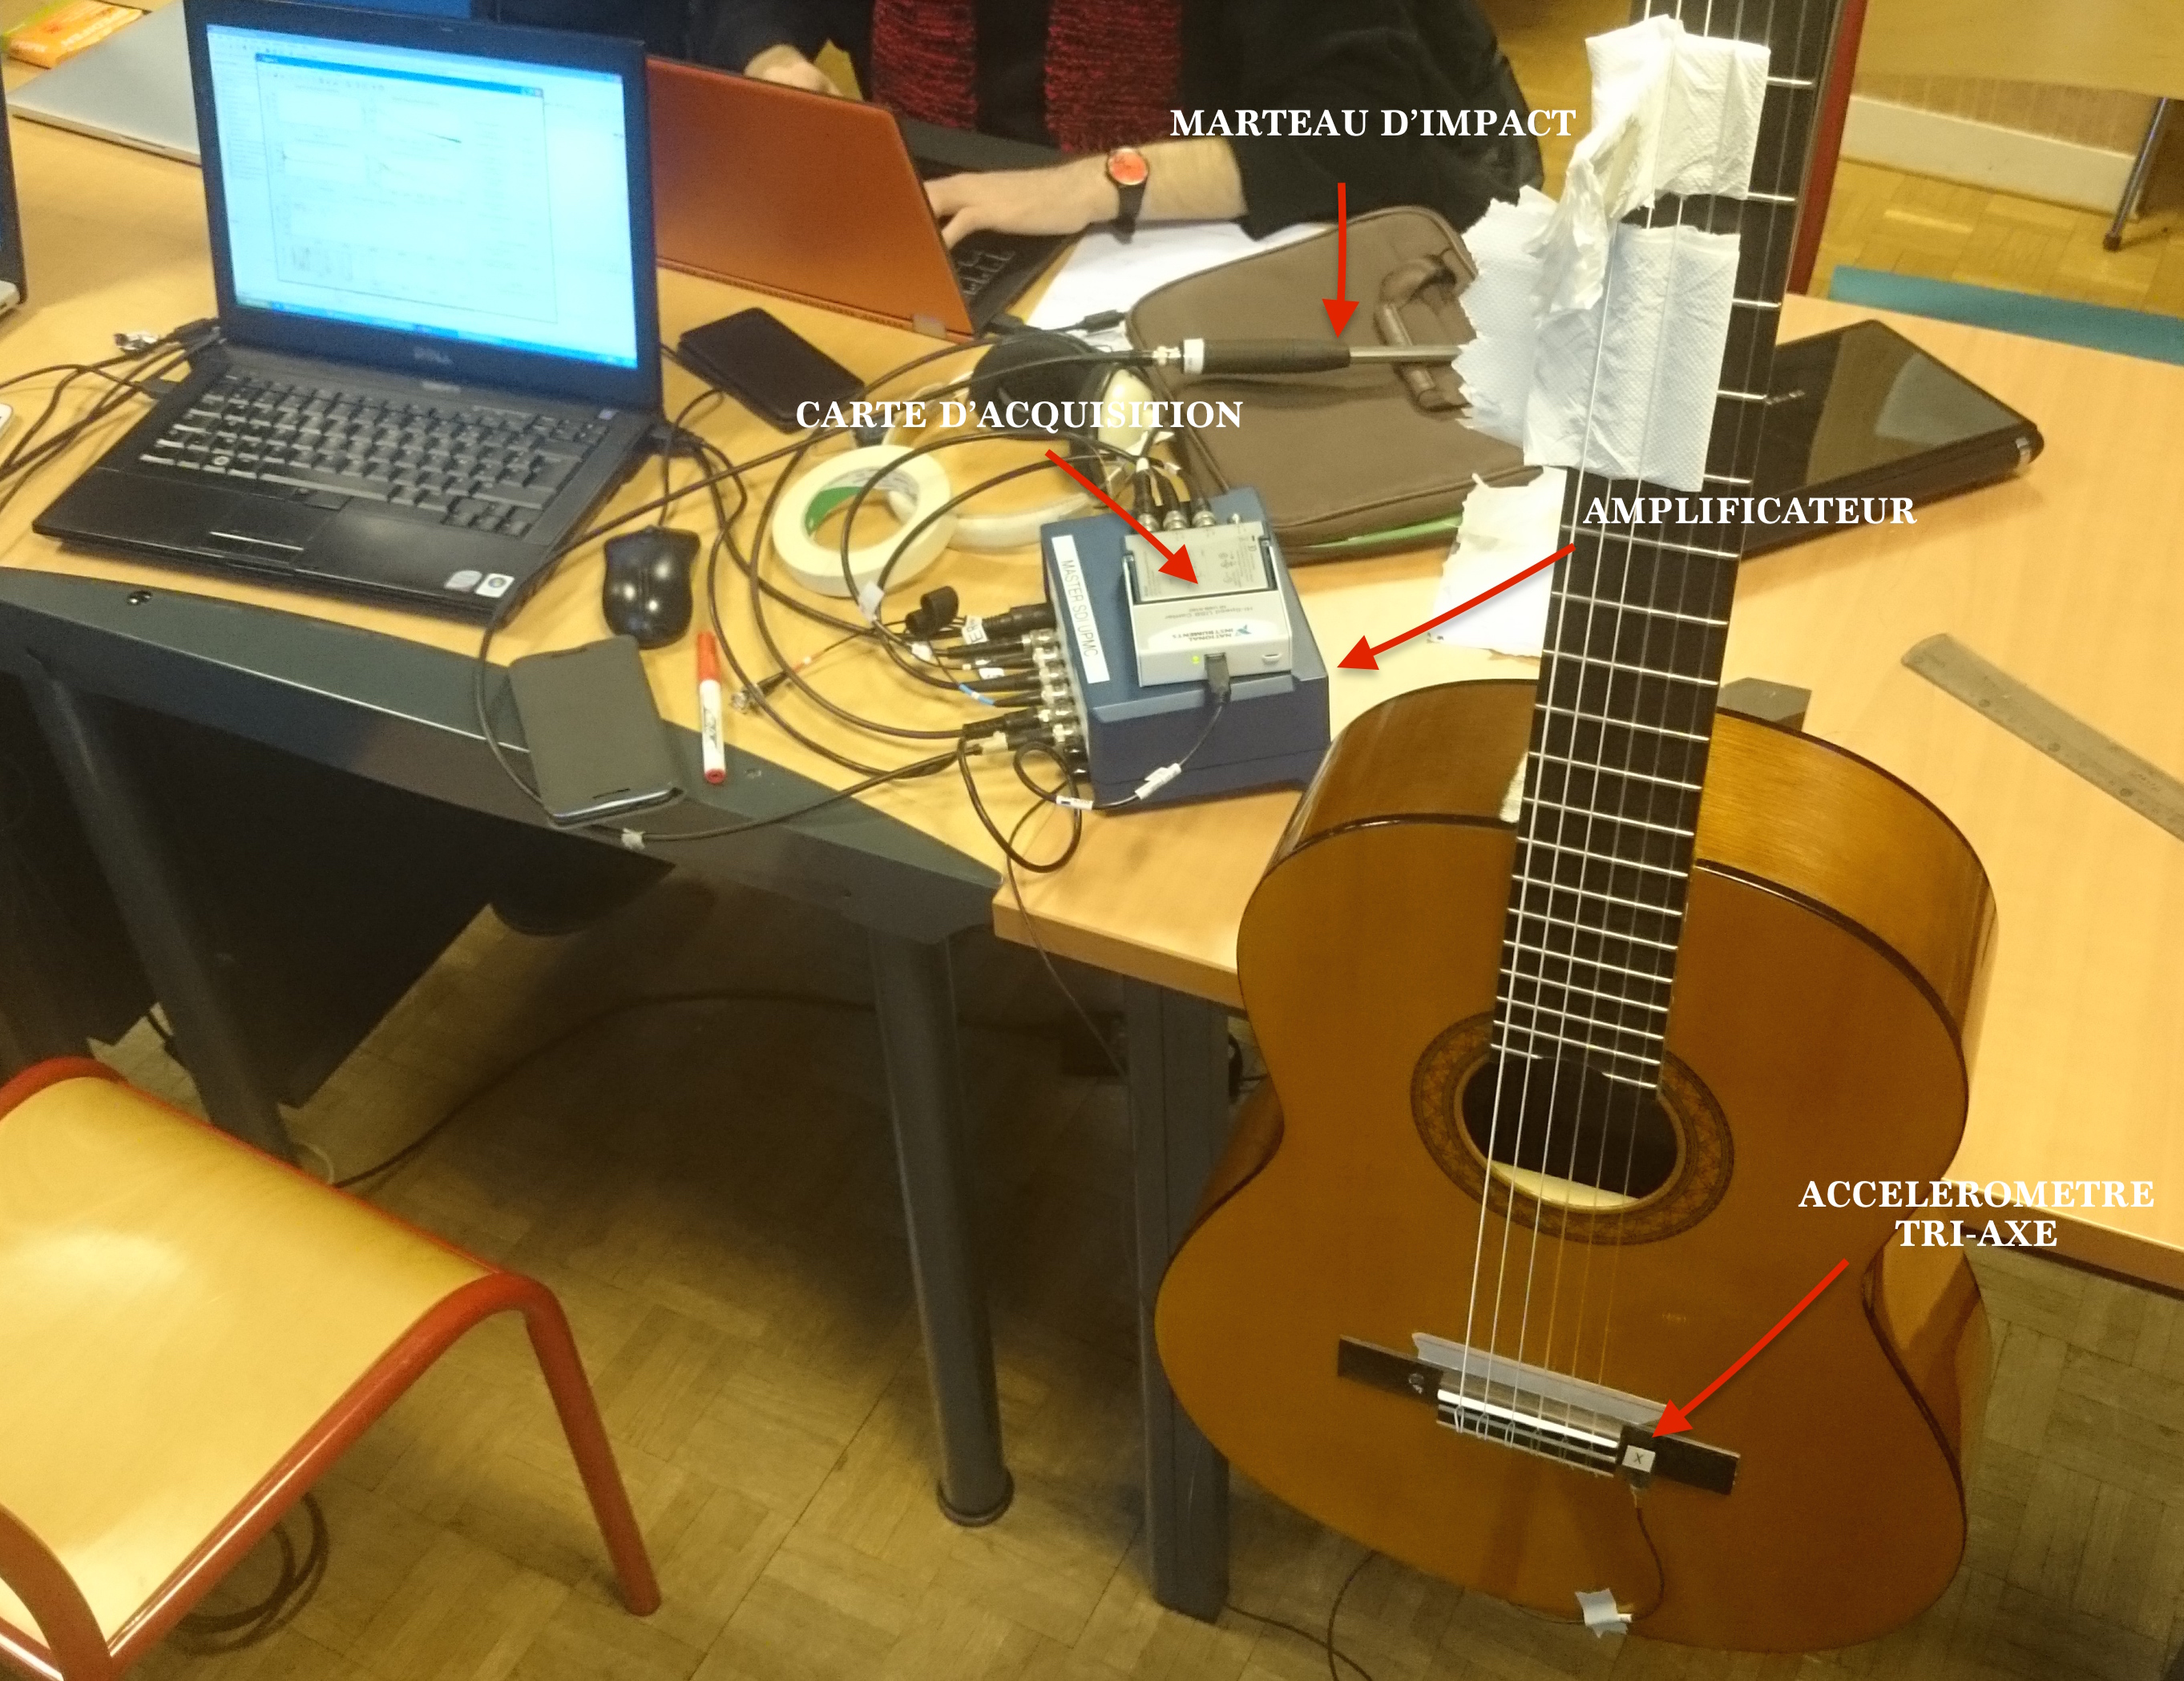
\includegraphics[width = 8cm]{figures/dispo.JPG}
\end{figure}
\end{frame}

 \begin{frame}{Protocole de mesure} 
  \begin{itemize}
  	\item Mesures d'admittance (accélération sur force) de corps et des deux cordes de Mi.
  	\item types d'excitation : marteau et fil de cuivre
    \item Etude de la cohérence mesure au marteau.
    \begin{figure}
		\centering
		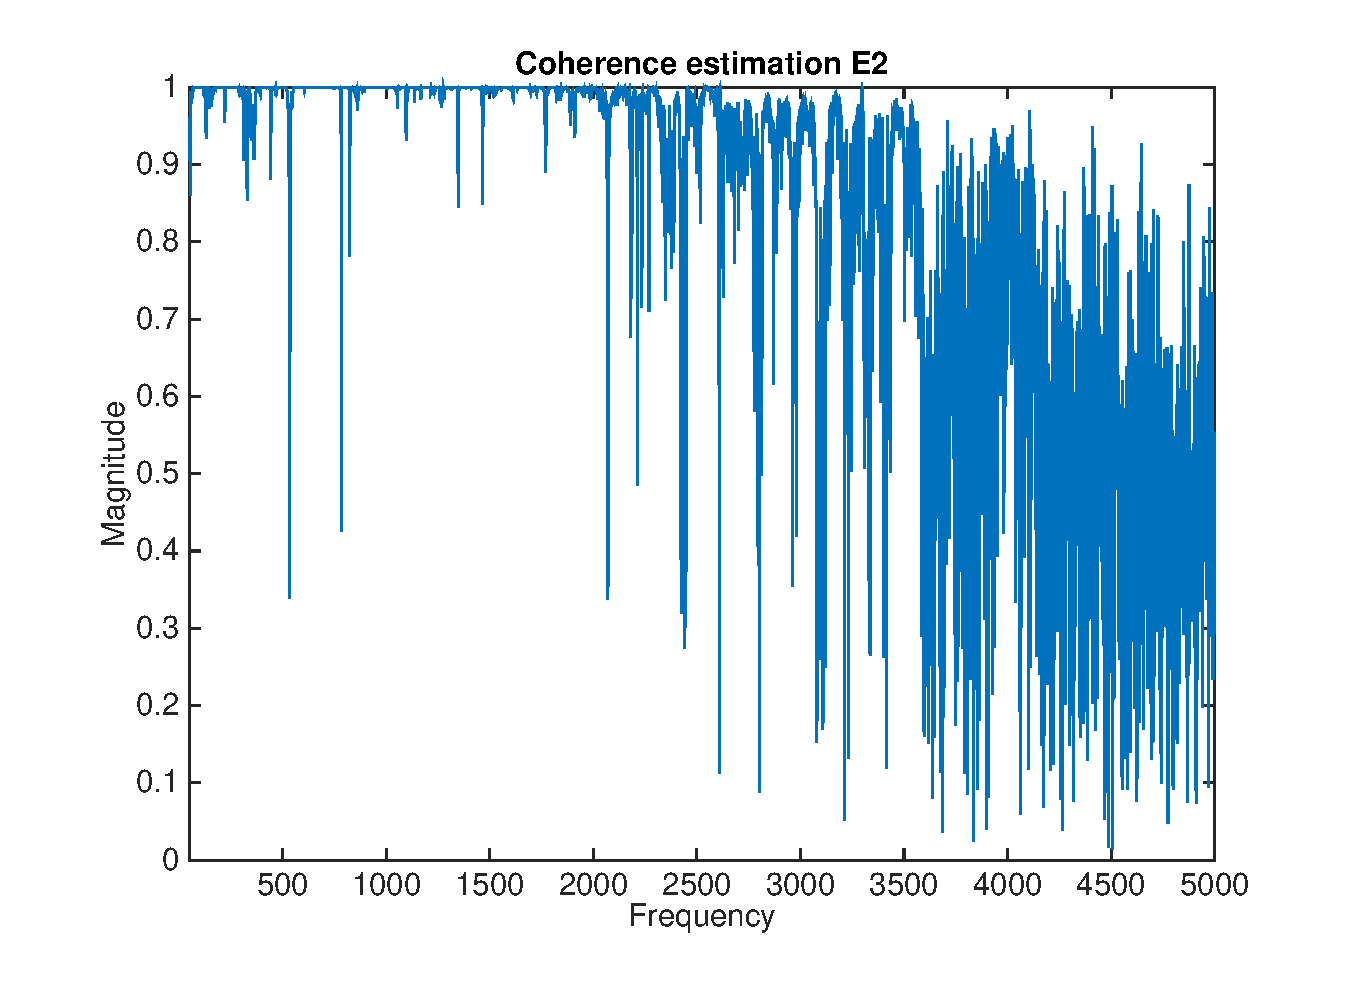
\includegraphics[width = 4.5cm]{figures/coherence_Z_1_E2.eps}
	\end{figure}
  
  \item Exploitation des résultats : 
  \begin{itemize}
  	\item acceleration, force, admittance
  	\item Application ESPRIT
  \end{itemize}
  \end{itemize} 
 \end{frame}